%!TEX root = ../msc_thesis.tex

\chapter{Machine learning}
\label{ch:machine_learning}



%%%%%%%%%%%%%%%%%%%%%%%%%%%%%%%%%%%%%%%%%%%%%%%%%%%%%%%%%%%%%%%%%%%%%%%%%%%%%%%%%%%%%%%%%%
%%%%%%%%%%%%%%%%%%%%%%%%%%%%%%%%%%%%%%%%%%%%%%%%%%%%%%%%%%%%%%%%%%%%%%%%%%%%%%%%%%%%%%%%%%
%%%
%%%%%%%%%%%%%%%%%%%%%%%%%%%%%%%%%%%%%%%%%%%%%%%%%%%%%%%%%%%%%%%%%%%%%%%%%%%%%%%%%%%%%%%%%%
%%%%%%%%%%%%%%%%%%%%%%%%%%%%%%%%%%%%%%%%%%%%%%%%%%%%%%%%%%%%%%%%%%%%%%%%%%%%%%%%%%%%%%%%%%

\section{Machine learning}

Machine learning is a set of methods used to learn patterns in data, and then use these patterns to take decisions, such as making predictions about new unseen data,  clustering, or have an agent taking actions based on a reward signal \cite{murphy2012machine} \cite{sutton1998reinforcement}. With the amount of data available nowadays, it has become a fruitful and demanded field in many areas. Machine learning has exploded lately mainly thanks to the advanced in computing power, without which most of modern techniques wouldn't be feasible.

Machine learning is usually divided in supervised learning, unsupervised learning and reinforcement learning. The first one involves building a model to predict a response variable from certain explanatory variables (or features). The second one involves a set of variables without a response in which one wishes to learn relationships and structure of the data. The third one involves mapping situations to actions to maximize a reward signal. Reinforcement learning (RL) is similar to supervised learning, but the biggest difference is that in RL, the learner is not told which actions it should take, it learns through trial and error.

An example of supervised learning is to estimate the income of a home from a set of variables such as zip code, size of home, number of cars they own, etc. An example of unsupervised learning is to find groups of homes that naturally come up in the data, such that there is high similarity within each group and little between groups. An example of RL is to learn to play the arcade game Pong. Recently, supervised learning and reinforcement learning have been combined to achieve harder goals, such as beating the Go world champion \cite{silver2017mastering} In this work, only supervised learning is presented and studied.

As previously mentioned, in supervised learning there is a response variable denoted as vector $y$ with $n$ elements, and each feature is denoted by $x^{(k)} \in \mathbb{R}^n$ for $k$ from 1 to $p$. All features can be summarized in notation in a single data matrix $X \in \mathbb{R}^{n \times p}$. It is assumed that there exists a relationship between $y$ and $X$, which can be written as
\begin{equation}
  \label{eq:general_learning_model}
  Y = f(X) + \varepsilon,
\end{equation}
where $f$ is a fixed but unknown function and $\varepsilon$ is a random error term, independent from $X$ and with zero mean \cite[p.~16]{james2013introduction}. The goal is usually to estimate function $f$, either prediction or inference, and this is done with an estimate $\hat{f}$ \cite[p.~17]{james2013introduction}.
In this work, the focus will be on the prediction goal.
The estimate $\hat{f}$ can be chosen from a wide family of models, such as a linear regression model, a general additive model, a neural network, etc., and the goal is for $\hat{f}$ have as little generalization error as possible. This is done using a training set of data, denoted $\mathcal{L} = \left\{ (x_1, y_1), ..., (x_n, y_n) \right\}$, and an error or loss function that needs to be minimized.

For example, in the linear regression case, it is common to minimize the squared error function
\begin{equation}
  \hat{f} = \argmin_{f \in \mathcal{F}} \frac{1}{n} \sum_{i = 1}^n{ ( y_i - f(x_i) ) ^ 2},
\end{equation}
where $\mathcal{F}$ is the family of functions of the form $f(X) = X\theta$ with $\theta \in \mathbb{R}^p$. Thus, the  estimate $\hat{f}$ is $\hat{f}(X) = X \hat{\theta}$, where $\hat{\theta}$ minimizes the error function.

The linear regression model belongs to a type of methods called \textbf{parametric methods}, in which the modeler first makes an assumption about the functional form of $f$, and then trains the model by choosing the parameters that minimize a previously selected loss function \cite[p.~21]{james2013introduction}. In the case of linear regression, the form of $f$ is assumed to be $f(X) = X\theta$, and the parameters chosen are the elements of the $\hat{\theta}$ vector that minimize the squared error function of the model.

An approach to the estimation of parameters that is different to the concept of error function minimization is the one of \textbf{maximum likelihood estimation}.
This is a probabilistic approach in which a certain probability distribution for the data is assumed.
In the case of linear regression, it is commonly assumed that the error term in \eqref{eq:general_learning_model} has a Gaussian distribution such that $\varepsilon_i \sim \normaldist{0}{\sigma^2}$, then $y_i \sim \normaldist{x_i^T \theta}{\sigma^2}$ for $i \in \left\{ 1, \ldots, n \right\}$. It is also usually assumed that the observations $y_i$ come from a random sample and are independent of each other. Therefore, the log-probability of the sample is
\begin{equation}
  \label{eq:gaussian_likelihood}
  %L(\theta) = \sum_{i = 1}^n \log \frac{1}{\sqrt{2 \pi \sigma^2}} e^{-\frac{(y_i - x_i^T \theta)^2}{2\sigma^2}},
  L(\theta) = \sum_{i = 1}^n \log \left[ \frac{1}{\sqrt{2 \pi \sigma^2}} e^{- \frac{(y_i - x_i^T \theta)^2}{2\sigma^2}} \right],
\end{equation}
%where $\normalfunc{x_i}{\mu}{\sigma^2}$ denotes the density function of a Gaussian random variable with mean $\mu$ and variance $\sigma^2$ evaluated in point $x_i$.

The \textbf{principle of maximum likelihood} states that the values for $\theta$ should be chosen so that the observed probability of the random sample is the highest, i.e., so that they maximize equation \eqref{eq:gaussian_likelihood} \cite[p.~31]{friedman2001elements} \cite[p.~303]{roussas1973first}.
With some algebra, it is fairly easy to see that maximizing equation \eqref{eq:gaussian_likelihood} is equivalent to minimizing the squared error loss.

In the case of a binary classification problem, assuming that $y_i$ follows a Bernoulli distribution, such that the probability of $y_i$ of being 1 is $p_i(\theta)$, where $\theta$ is the parameter that indexes the probability, then the likelihood function in this case is $\prod_{i = 1}^n  p_i(\theta)^{y_i}\left(1 - p_i(\theta) \right)^{1 - y_i}$ and thus, the log-likelihood is
\begin{equation}
  L(\theta) = \sum_{i = 1}^n \left[ y_i \log\left( p_i(\theta) \right) + (1 - y_i) \log \left( 1 - p_i(\theta) \right) \right].
\end{equation}

Another approach to the learning problem is the \textbf{Bayesian approach}, in which a prior distribution on the parameters $\theta$ is assumed, and then the knowledge about them is updated with data. That is, the modeler first quantifies the knowledge that they may have about $\theta$ using a prior distribution $\prob{\theta}$ and then computes the posterior distribution of $\theta$ given $X$ and $y$ using Bayes' theorem as such
\begin{equation}
  \label{eq:bayes_theorem}
  \prob{\theta | y, X } = \frac{\prob{y | \theta, X} \prob{\theta | X}}{\prob{y | X}} = \frac{\prob{y | \theta, X} \prob{\theta | X}}{\int \prob{y | \theta, X} \prob{\theta | X} d\theta}.
\end{equation}

The posterior distribution represents the knowledge about $\theta$ after the data has been seen. It is a compromise between the prior beliefs and the data. % The multiplier $\prob{y | \theta, X}$ is called the likelihood, and is the probability of the data given the parameters.

Since the denominator of equation \eqref{eq:bayes_theorem} does not depend on $\theta$ because it is only a normalizing constant, it is just usually described as a proportion
\begin{equation}
  \label{eq:bayes_theorem_prop}
    \prob{\theta | y, X} \propto \prob{y | \theta, X} \prob{\theta | X}.
\end{equation}

The posterior distribution is also used to predict the values of unseen data. Let $x^*$ be a vector of features for which a prediction $\hat{y}^*$ is desired, then the \textbf{posterior predictive distribution} must be used, defined as
\begin{equation}
  \label{eq:post_pred_dist}
  \prob{y^* | X, y, x^*} = \int \prob{y^* | \theta, x^*} \prob{\theta | X, y} d\theta.
\end{equation}

Note that this posterior distribution is, as it name implies, a distribution, i.e., it is not a single prediction but many predictions, possibly an infinite number, weighted by how probable each value is to be. If the goal is to have a point prediction $\hat{y}^*$ for $x^*$, then the modeler could use decision theory to find a point estimate. The idea is to specify a loss function $L(y^*, \hat{y}^*)$ that quantifies the loss of having an estimate $\hat{y}^*$ when the real value is $y^*$, and have the point estimate be the $\hat{y}^*$ that minimizes this loss function. The optimal value for the squared loss $L(y^*, \hat{y}^*) = (y^* - \hat{y}^*)^2$ is the expected value of the posterior predictive distribution, that is,
\begin{equation}
  \hat{y}^* = \mathbb{E}_{y^* | x^*, y, X} \left[ \prob{y^* | X, y, x^*} \right].
\end{equation}

Another loss function is the absolute loss $L(y^*, \hat{y}^*) = \vert y^* - \hat{y}^* \vert$ which results in using the median of the posterior predictive distribution as a point estimate. One more function is the 0-1 loss function $L(y^*, \hat{y}^*) = \mathbb{I}(y^* \neq \hat{y}^* )$ which results in using the mode of the posterior predictive distribution as a point estimate. This last estimate is also called a maximum a posteriori estimate.

\subsection{Example}

All these concepts can be illustrated in the context of logistic regression. Suppose that we have $n$ observations of a binary response variable $y \in \left\{0, 1\right\}^n$ and two continuous features $x^{(1)}, x^{(2)} \in \mathbb{R}^n$. The frequentist approach using the maximum likelihood estimate will be studied first, then it will be transformed into a simple learning problem in which the goal is to minimize a loss function, and finally, the Bayesian approach will be examined.

If someone wanted to build a classifier using a linear regression model, then they would run into a problem because a linear model of the form $\mu(x_i) = \theta_0 + \theta_1 x_i^{(1)} + \theta_2 x_i^{(2)}$ is not bounded. In contrast, the response variable $y$ from the data only takes the values $0$ and $1$, hence, it is a better idea to model the probability that a feature vector belongs to each class. This way, $y_i$ is a random variable that follows a Bernoulli distribution with parameter $p_i$, where $p_i$ is the probability of $y_i$ being 1.
The range of $f$ as a linear model is $\mathbb{R}$, so it must be mapped to the $\left[ 0,1 \right]$ interval in which probabilities live, and it can be done with what is called a \textbf{link function}. The \textbf{logistic sigmoid function} % $\sigma \left( \cdot \right)$
is a widely used link function for this type of problems \cite[p.~114]{christopher2006pattern}. It is defined as
\begin{equation}
  \sigma(w) = \frac{e^w}{1 + e^w} = \frac{1}{1 + e^{-w}}.
\end{equation}

It is easy to see that $\lim_{w \to -\infty} \sigma(w) = 0$ and $\lim_{w \to \infty} \sigma(w) = 1$. 

%There is more reasoning behind the logistic sigmoid function, and some of it has to be that it belongs to the exponential family of functions. For more details about this, see \cite{christopher2006pattern}.

Another possible link function is the \textbf{probit function}, defined as the inverse of the cumulative distribution function of a Gaussian random variable \cite[p.~296]{friedman2001elements}. That is, $\sigma(w) = \Phi^{-1}\left( x \right)$,
where
\begin{equation}
  %\Phi(w) = \int_{-\infty}^w \frac{1}{\sqrt{2 \pi}} \exp{\left( -\frac{x^2}{2} \right)} dx = \int_{-\infty}^w \normalfunc{x}{0}{1} dx.
  \Phi(w) = \int_{-\infty}^w \frac{1}{\sqrt{2 \pi}} \exp{\left( -\frac{x^2}{2} \right)} dx.
\end{equation}

There are some differences in the theory and behavior of the logistic and the probit functions, but in practice they hardly make any substantial difference and the choice of one over the other may be a matter of taste or convenience \cite[p.~118]{gelman2006data}. Henceforth, we will use the logistic function as the link function for binary classification problems.

It has been established that $\sigma \left( \cdot \right)$ maps from $\mathbb{R}$ to $\left[ 0,1 \right]$, but it is yet to be explained how to relate this to the original problem which is to build a linear classifier using the vectors $x^{(1)}$ and $x^{(2)}$. Using  $\sigma \left( \cdot \right)$, one can define the probability that $y_i$ belongs to class $1$ given features $x_i^{(1)}$ and $x_i^{(2)}$ as
\begin{equation}
  \prob{y_i = 1 | x_i, \theta} = \sigma(\theta_0 + \theta_1 x_i^{(1)} + \theta_2 x_i^{(2)}) = \frac{1}{1 + e^{-\left( \theta_0 + \theta_1 x_i^{(1)} + \theta_2 x_i^{(2)} \right)}},
\end{equation}
with $x_i = \left[ x_i^{(1)}, x_i^{(2)} \right]^T$. Thus
\begin{equation}
  \prob{y_i = 0 | x_i, \theta} = 1 - \prob{y_i = 1 | x_i} = \frac{1}{1 + e^{\theta_0 + \theta_1 x_i^{(1)} + \theta_2 x_i^{(2)}}}.
\end{equation}

This means that $y_i$ is fully described as a Bernoulli distribution with parameter $p_i =\prob{y_i = 1 | x_i, \theta}$. When the response variable is Bernoulli distributed, the likelihood of $n$ independent observations is
\begin{equation}
  \prod_{i = 1}^n  p_i(\theta)^{y_i}\left(1 - p_i(\theta) \right)^{1 - y_i}.
\end{equation}

Then, in consequence, the log-likelihood of $n$ independent observations is
\begin{equation}
  \label{eq:log_likelihood_logistic_example}
  L(\theta) = \sum_{i = 1}^n \left[ y_i \log\left( p_i(\theta) \right) + (1 - y_i) \log \left( 1 - p_i(\theta) \right) \right],
\end{equation}
where $p_i(\theta) = \sigma(\theta_0 + \theta_1 x_i^{(1)} + \theta_2 x_i^{(2)})$.

The maximum likelihood estimator of $\theta = \left[ \theta_0, \theta_1, \theta_2 \right]^T$ is the vector $\hat{\theta}$ that maximizes $L(\theta)$ in equation \eqref{eq:log_likelihood_logistic_example}; that is $\hat{\theta} = \argmax L(\theta)$.

Another way to interpret the problem of binary classification, is to consider the learning problem from an optimization perspective in which the goal is to minimize a certain loss function. It has been shown above that maximizing equation \eqref{eq:log_likelihood_logistic_example} leads to the maximum likelihood estimate. However, if the sign is changed, the result is a loss function that can be minimized, and it is the exact same problem as before.

The new objective function that needs to be minimized is
\begin{equation}
  \label{eq:logistic_example_loss_function}
  L(\theta) = - \sum_{i = 1}^n \left[ y_i \log\left( p_i(\theta) \right) + (1 - y_i) \log \left( 1 - p_i(\theta) \right) \right].
\end{equation}

Intuitively, this is an error function because if $y_i = 1$, then $1 - y_i = 0$, so the second term in the loss function vanishes and what is left remaining is $\log\left( p_i(\theta) \right)$. Now, when $p_i(\theta)$ is big, that is, close to 1, then $\log\left( p_i(\theta) \right) \to 0$. However, if $p_i(\theta)$ is small, that is, close to 0, then $\log\left( p_i(\theta) \right) \to -\infty$, and so the overall loss function tends to infinity. This means that when the real value of $y_i$ is 1 and a low probability is assigned to it, then the loss function is large; but if a high probability is assigned to it, then the loss function is small. The same reasoning works for when $y_i = 0$.
% The same reasoning works for when $y_i = 0$: if a low probability is assigned, then the loss function is small; but if a high probability is assigned, then the loss function is large. 
Hence, minimizing the loss function leads to choosing values of $\theta$ that yield a high probability to the cases when $y_i = 1$ and a low one when $y_i = 0$.

% There are other possible loss functions for this problem, such as the \textbf{hinge loss}

The logistic regression model can be reformulated from a Bayesian approach. As before, it will be assumed that $y_i$ follows a Bernoulli distribution such that the probability of being 1 is $p_i(\theta) = \sigma(\theta_0 + \theta_1 x_i^{(1)} + \theta_2 x_i^{(2)})$, where $\sigma \left( \cdot \right)$ is the logistic sigmoid function. In the Bayesian paradigm, the unknown parameter vector $\boldsymbol{\theta} = \left[ \theta_0, \theta_1, \theta_2 \right]^T$ must have a joint prior distribution. A good idea is to assume a Gaussian distribution for the unknown unobservable parameter $\boldsymbol{\theta}$. Furthermore, independence between the components of $\boldsymbol{\theta}$ can be assumed which in turn allows one to write the prior distribution as
\begin{equation}
  %\theta \sim \normaldist{\mu}{\frac{1}{\tau} I},
  \theta \sim \normaldist{\mu}{\sigma^2 I},
\end{equation}
where $\mu \in \mathbb{R}^3$, $\sigma^2 \in \mathbb{R}^+$ and $I$ is a $3 \times 3$ identity matrix. 
% In this context, $\tau$ is the inverse of the variance, and is called the \textbf{precision}. 
Assuming $\mu = \left[ \mu_0, \mu_1, \mu_2 \right]^T$, then the prior distribution takes the following form
\begin{equation}
  % \prob{\theta} = \prod_{k = 0}^2 \sqrt{\frac{\tau}{2 \pi}} e^{- \tau \frac{\left( \theta_k - \mu_k \right)^2}{2}}.
  \prob{\theta} = \prod_{k = 0}^2 \frac{1}{\sqrt{2 \pi \sigma^2}} e^{- \frac{(\theta_k - \mu_k)^2}{2\sigma^2}}.
\end{equation}

The likelihood can be written as
\begin{equation}
  \prob{X | \theta} = \prod_{i = 1}^n  p_i(\theta)^{y_i}\left(1 - p_i(\theta) \right)^{1 - y_i},
\end{equation}
which follows from the independence assumption in the data-generating mechanism. Furthermore, Bayes' theorem in equation \eqref{eq:bayes_theorem_prop} allows one to write the posterior distribution as
%so, following Bayes' theorem in equation \eqref{eq:bayes_theorem_prop}, the posterior distribution is
\begin{equation}
  \prob{\theta | y, X} =
    \frac
    {
      \left[ \prod_{i = 1}^n  p_i(\theta)^{y_i}\left(1 - p_i(\theta) \right)^{1 - y_i} \right]
      \left[ \prod_{k = 0}^2 \frac{1}{\sqrt{2 \pi \sigma^2}} e^{- \frac{(\theta_k - \mu_k)^2}{2\sigma^2}} \right]
      % \left[ \prod_{k = 0}^2 \sqrt{\frac{\tau}{2 \pi}} e^{- \tau \frac{\left( \theta_k - \mu_k \right)^2}{2}} \right]
    }{
      \int \left[ \prod_{i = 1}^n  p_i(\theta)^{y_i}\left(1 - p_i(\theta) \right)^{1 - y_i} \right]
      \left[ \prod_{k = 0}^2 \frac{1}{\sqrt{2 \pi \sigma^2}} e^{- \frac{(\theta_k - \mu_k)^2}{2\sigma^2}} \right]
      % \left[ \prod_{k = 0}^2 \sqrt{\frac{\tau}{2 \pi}} e^{- \tau \frac{\left( \theta_k - \mu_k \right)^2}{2}} d\theta
    }.
\end{equation}

Unfortunately, the integral cannot be solved analytically, which is why numerical methods are used. 
It should be noted that the denominator is a constant with respect to $\theta$, thus, the posterior distribution can be computed up to a normalizing constant as
%Most of them rely on the fact that the denominator is only a normalizing constant and only use the equation as a proportion
\begin{equation}
  \prob{\theta | y, X} \propto
  \left[ \prod_{i = 1}^n  p_i(\theta)^{y_i}\left(1 - p_i(\theta) \right)^{1 - y_i} \right]
  \left[ \prod_{k = 0}^2 \frac{1}{\sqrt{2 \pi \sigma^2}} e^{- \frac{(\theta_k - \mu_k)^2}{2\sigma^2}} \right].
  %\left[ \prod_{k = 0}^2 \sqrt{\frac{\tau}{2 \pi}} e^{- \tau \frac{\left( \theta_k - \mu_k \right)^2}{2}} \right].
\end{equation}

Methods to estimate the posterior include Markov Chain Monte Carlo (MCMC) methods such as Metropolis-Hastings or Hamiltonian Monte Carlo, and Variational Inference, discussed in chapter \ref{ch:variational_inference}.

No matter what paradigm one follows, in general, when one is training a model for prediction, it is not the main goal to minimize training error, but prediction error, i.e., the error of any future observation $(x^*, y^*)$. This means that one wants to minimize the expected prediction error, hence, it is common to divide the data set $(X, Y)$ in two: the training set and the test set. To do this, from the original data set, a random sample of observations is assigned to be part of the training set and the rest are part of the test set. The idea is that the test set should be used to measure the predictive performance of the model. A third set is sometimes added and is called the validation set, in which predictive performance is measured to select certain hyperparameters, such as regularization parameter values, discussed further in this document.


%%%%%%%%%%%%%%%%%%%%%%%%%%%%%%%%%%%%%%%%%%%%%%%%%%%%%%%%%%%%%%%%%%%%%%%%%%%%%%%%%%%%%%%%%%
%%%%%%%%%%%%%%%%%%%%%%%%%%%%%%%%%%%%%%%%%%%%%%%%%%%%%%%%%%%%%%%%%%%%%%%%%%%%%%%%%%%%%%%%%%
%%% Loss function optimization
%%%%%%%%%%%%%%%%%%%%%%%%%%%%%%%%%%%%%%%%%%%%%%%%%%%%%%%%%%%%%%%%%%%%%%%%%%%%%%%%%%%%%%%%%%
%%%%%%%%%%%%%%%%%%%%%%%%%%%%%%%%%%%%%%%%%%%%%%%%%%%%%%%%%%%%%%%%%%%%%%%%%%%%%%%%%%%%%%%%%%

\section{Loss function optimization}

As mentioned before, in machine learning the goal is to find the parameters that minimize a loss function such as the one in equation \eqref{eq:logistic_example_loss_function}. In some cases like linear regression, it is possible to use the first and second order conditions to find a closed formula to find the parameters; but in many other cases this cannot be done, like in logistic regression, so we resort to numerical optimization techniques. The general problem of unrestricted optimization \cite{nocedal2006numerical} is
\begin{equation}
  \min_{\theta \in \mathbb{R}^p} L(\theta).
\end{equation}

In machine learning, $L$ is usually a convex loss function and $\theta$ is a parameter or vector of parameters. A solution is a vector $\theta^*$ called local minimizer, which minimizes the function $L$ in a neighborhood around $\theta^*$. Formally, a vector $\theta^*$ is a local minimizer if there exists a neighborhood $\mathcal{V}$ of $\theta^*$ such that $L(\theta^*) \leq L(\theta)$ for all $\theta \in \mathcal{V}$.

The sufficient second order conditions are used in numerical optimization. Suppose that the Hessian matrix $\nabla^2 L$ is continuous in an open neighborhood of $\theta^*$, that the gradient $\nabla L(\theta^*) = 0$ and that $\nabla^2 L(\theta^*)$ is positive definite; then $\theta^*$ is a local minimizer of $L$.

This is basic calculus, but it provides the base of numerical optimization algorithms. In general, all algorithms search for a point $\theta^*$ such that $\nabla L(\theta^*) = 0$.

\subsection{Gradient descent (GD)}

Generally, numerical optimization algorithms are iterative, and gradient descent belongs to this class. Particularly, it belongs to a family called \textbf{line search algorithms}. In each iteration, the algorithms search for a direction in which to move and then update the current value in accordance to that direction. That is, in the $k$-th iteration, $\theta$ has the value $\theta_k$, and the algorithms look for a direction $p_k$ to update to a new value $\theta_{k+1} = \theta_k + \alpha_k p_k$, where $\alpha_k > 0$ is the ``distance'' in which the algorithm moves toward direction $p_k$, and is called \textbf{step length}. Once that the value of the parameter is updated, the algorithm finds a new direction in which to move forward and then updates the parameter value again. This is done until a stopping criteria is met, this usually being that the gradient vector norm is smaller than a certain small positive scalar.

In gradient descent, the direction $p_k$ in which the algorithm moves is the maximum descent direction, that is, the negative of the gradient $-\nabla L(\theta_k)$. So, in each iteration $\theta$ is updated as such
\begin{equation}
  \label{eq:parameter_update_gd}
  \theta_{k+1} = \theta_k - \alpha_k \nabla L(\theta_k).
\end{equation}

Choosing the step length $\alpha_k$ is problematic because it is desirable to find a value such that the function $L$ decreases as much as possible, but it is not desirable to spend too much time choosing the value.
%The best option is the global minimizer of the auxiliary function $\phi(\alpha_k) = L(\theta_k + \alpha_k p_k)$, but it is too expensive to compute.
Generally, heuristics are used to choose the sequence of values for $\alpha_k$, such as using the outer product of the gradient with itself, as shown in \cite{duchi2011adaptive}.

Now, let's study how gradient descent works in the case of logistic regression. The loss function to be minimized, defined in equation \eqref{eq:logistic_example_loss_function}, is
\begin{equation}
  L(\theta) = - \sum_{i=1}^{n} \left[ y_i \log(\sigma(\theta^T x_i)) + (1-y_i) \log(1-\sigma(\theta^T x_i)) \right] =
  - \sum_{i=1}^{n}{\ell_i(\theta)}
\end{equation}
where $\sigma(\cdot)$ is the logistic sigmoid function, $\theta^T x_i = \sum_{j=0}^{p}{\theta_j x_{ij}}$, $x_{i1} = 1$ for all $i \in \left\{1, ..., n \right\}$ and $\ell_i(\theta)$ is defined as
\begin{equation}
  \ell_i(\theta) = y_i \log(\sigma(\theta^T x_i)) + (1-y_i) \log(1-\sigma(\theta^T x_i)).
\end{equation}

Taking the partial derivatives of the loss function with respect to the parameters the result is
\begin{equation}
  \frac{\partial L}{\partial \theta_j} = - \sum_{i = 1}^n { \frac{\partial \ell_i}{\partial \theta_j} }
\end{equation}
and, using the fact that $\sigma'(w) = \sigma(w)(1-\sigma(w))$, then each partial derivative from the sum
\begin{equation}
  \begin{split}
    \frac{\partial \ell_i}{\partial \theta_j} & =
    \frac{y_i \sigma'(\theta^T x_i) x_{ij} }  {\sigma(\theta^T x_i)} + \frac{(1 - y_i) (-1) \sigma'(\theta^T x_i) x_{ij}} {1 - \sigma(\theta^T x_i)} \\
    & = \frac{\sigma'(\theta^T x_i) x_{ij} y_i}{\sigma(\theta^T x_i)} - \frac{(1 - y_i) \sigma'(\theta^T x_i) x_{ij}}{1 - \sigma((\theta^T x_i))} \\
    & = \sigma'(\theta^T x_i) x_{ij} \left(\frac{y_i}{\sigma(\theta^T x_i)} - \frac{1-y_i}{1-\sigma(\theta^T x_i)} \right) \\
    & = \sigma'(\theta^T x_i) x_{ij} \left(\frac{y_i - y_i \sigma(\theta^T x_i) -
    \sigma(\theta^T x_i) + y_i \sigma(\theta^T x_i)}{\sigma(\theta^T x_i)(1-\sigma(\theta^T x_i))} \right) \\
    & = x_{ij}(y_i - \sigma(\theta^T x_i)).
  \end{split}
\end{equation}

So, finally, the partial derivative is
\begin{equation}
  \frac{\partial L}{\partial \theta_j} = - \sum_{i = 1}^n { x_{ij}(y_i - \sigma(\sum_{j=0}^{p}{\theta_j x_{ij}})) }.
\end{equation}

Hence, the gradient descent direction for each iteration is
\begin{equation}
  \nabla_{\theta} L = \left( \frac{\partial L}{\partial \theta_1}, ..., \frac{\partial L}{\partial \theta_p} \right)^T.
\end{equation}

To minimize the loss function, an initial vector of parameters $\theta^0 \in \mathbb{R}^2$ is chosen, and in each iteration this vector is updated using equation \eqref{eq:parameter_update_gd} until certain criteria are met.

This algorithm was implemented in the R programming language by generating a vector $x \in \mathbb{R}^n$ with $n = 1000$ such that $x_i \sim N(0, 1)$ for each $i \in \left\{1, ..., n \right\}$; then an auxiliary vector was computed, $p_i = \frac{1}{\exp \left( - \theta_0 - \theta_1 x_i \right)}$, with $\theta_0 = -5$ and $\theta_1 = 5$. Finally, the response variable $y$ was built simulating Bernoulli random variables, such that $y_i \sim \mathrm{Bern}(p_i)$.
The implementation is compared with the result of the \texttt{glm} package.

The initial vector of parameters was $\theta^0 = (0, 0)^T$ and a constant value of $\alpha_k = 2$ was used. The stopping criteria was that the norm of the gradient $\nabla_{\theta} L(\theta)$ should be less than $0.0001$, which was achieved after 409 iterations.

Figure \ref{fig:GD_plots} shows the results of the implementation. On the left, the value of the loss function in each iteration can be seen. On the right, the parameter vector's value in each iteration. The red dot is the value of the estimate by the \texttt{glm} package. It can be seen that the implemented algorithm converges to this value.

\begin{figure}[H]
    \centering
    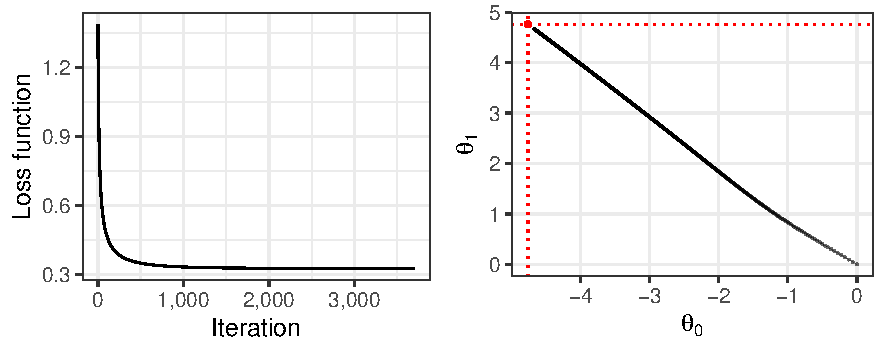
\includegraphics[width=\textwidth]{GD_plots.pdf}
    \caption{Example of gradient descent for logistic regression.}
    \label{fig:GD_plots}
\end{figure}

\subsection{Stochastic gradient descent (SGD)}

In machine learning it is common to find the need to solve optimization problems of the form
\begin{equation}
  \min_{\theta \in \mathbb{R}^p} L(\theta), \quad \text{with} \, \,
  L(\theta) = \frac{1}{n} \sum_{i = 1}^n { \ell_i(\theta) }.
\end{equation}

That is, the loss function that needs to be minimized is usually a sum or average of several indexed functions in which each indexed function depends only on one observation of the data set. For example, in logistic regression, the loss function that is expressed in that way.

Gradient descent uses iterations in the form
\begin{equation}
  \theta_{k+1} = \theta_k - \alpha_k \nabla L(\theta_k) :=\theta_k - \frac{\alpha_k}{n} \sum_{i = 1}^n \nabla \ell_i(\theta_k),
\end{equation}
which involves evaluating $n$ gradients (one for each observation) and then taking an average. In some cases of machine learning, $n$ can be really big; hence computing all of those gradients in each iteration is expensive. That is why researchers come up with methods such as SGD, in which the number of gradients to compute does not depend on $n$ and is constant instead. SGD uses iterations of the form
\begin{equation}
  \theta_{k+1} = \theta_k - \alpha_k \nabla \ell_{i_k}(\theta_k),
\end{equation}
where $i_k \in \left\{1, 2, ..., n \right\}$ is randomly chosen. The gradient $\nabla \ell_{i_k}(\theta_k)$ is an unbiased estimator of $\nabla L(\theta_k)$. This way, each iteration is really cheap because it involves the computation of only one gradient. It can happen that some $\nabla \ell_{i_k}(\theta_k)$ in particular does not give a direction of descent from $\theta_k$, but on average they yield descent directions, such that the sequence $\left\{ \theta_0, \theta_1, ... \right\}$ leads to a minimizer $\theta^*$.

\subsection{Mini-batch gradient descent}

An approach that is in between the two extremes of computing the gradients of all observations and the gradient of just one observation is \textbf{mini-batch gradient descent}. In mini-batch gradient descent, one chooses a fixed integer $l$, then the data set is divided in batches if size $l$, where the values in each batch are randomly chosen. Then, each of these batches is used to compute the gradient and update the values of the parameters. Usually $l$ is a small number compared to the size of a big data set, but big enough so that the gradient estimation is not too noisy, such as $l = 32$ or $l = 100$. This way, each iteration is cheaper because it involves the computation of only $l$ gradients instead of $n$. Stochastic gradient descent (SGD) is just mini-batch gradient descent with $l = 1$.

So, mini-batch gradient descent updates the value of the parameters in each iteration as such
\begin{equation}
  \theta_{k+1} = \theta_k - \frac{\alpha_k}{n} \sum_{i = 1}^l \nabla \ell_i(\theta_k).
\end{equation}

We implemented mini-batch gradient descent for logistic regression in R and test it with the same simulated data set as in the previous example. Figure \ref{fig:Mini-batch_GD_plots} shows the results of the implementation. Each of the plots shows the values of the parameters in each iteration, but the difference in each plot is the size of the mini-batch $l$. It is clear that with bigger $l$, the descent directions are less noisy, but in the end they all converge to more or less the same value.

\begin{figure}[H]
    \centering
    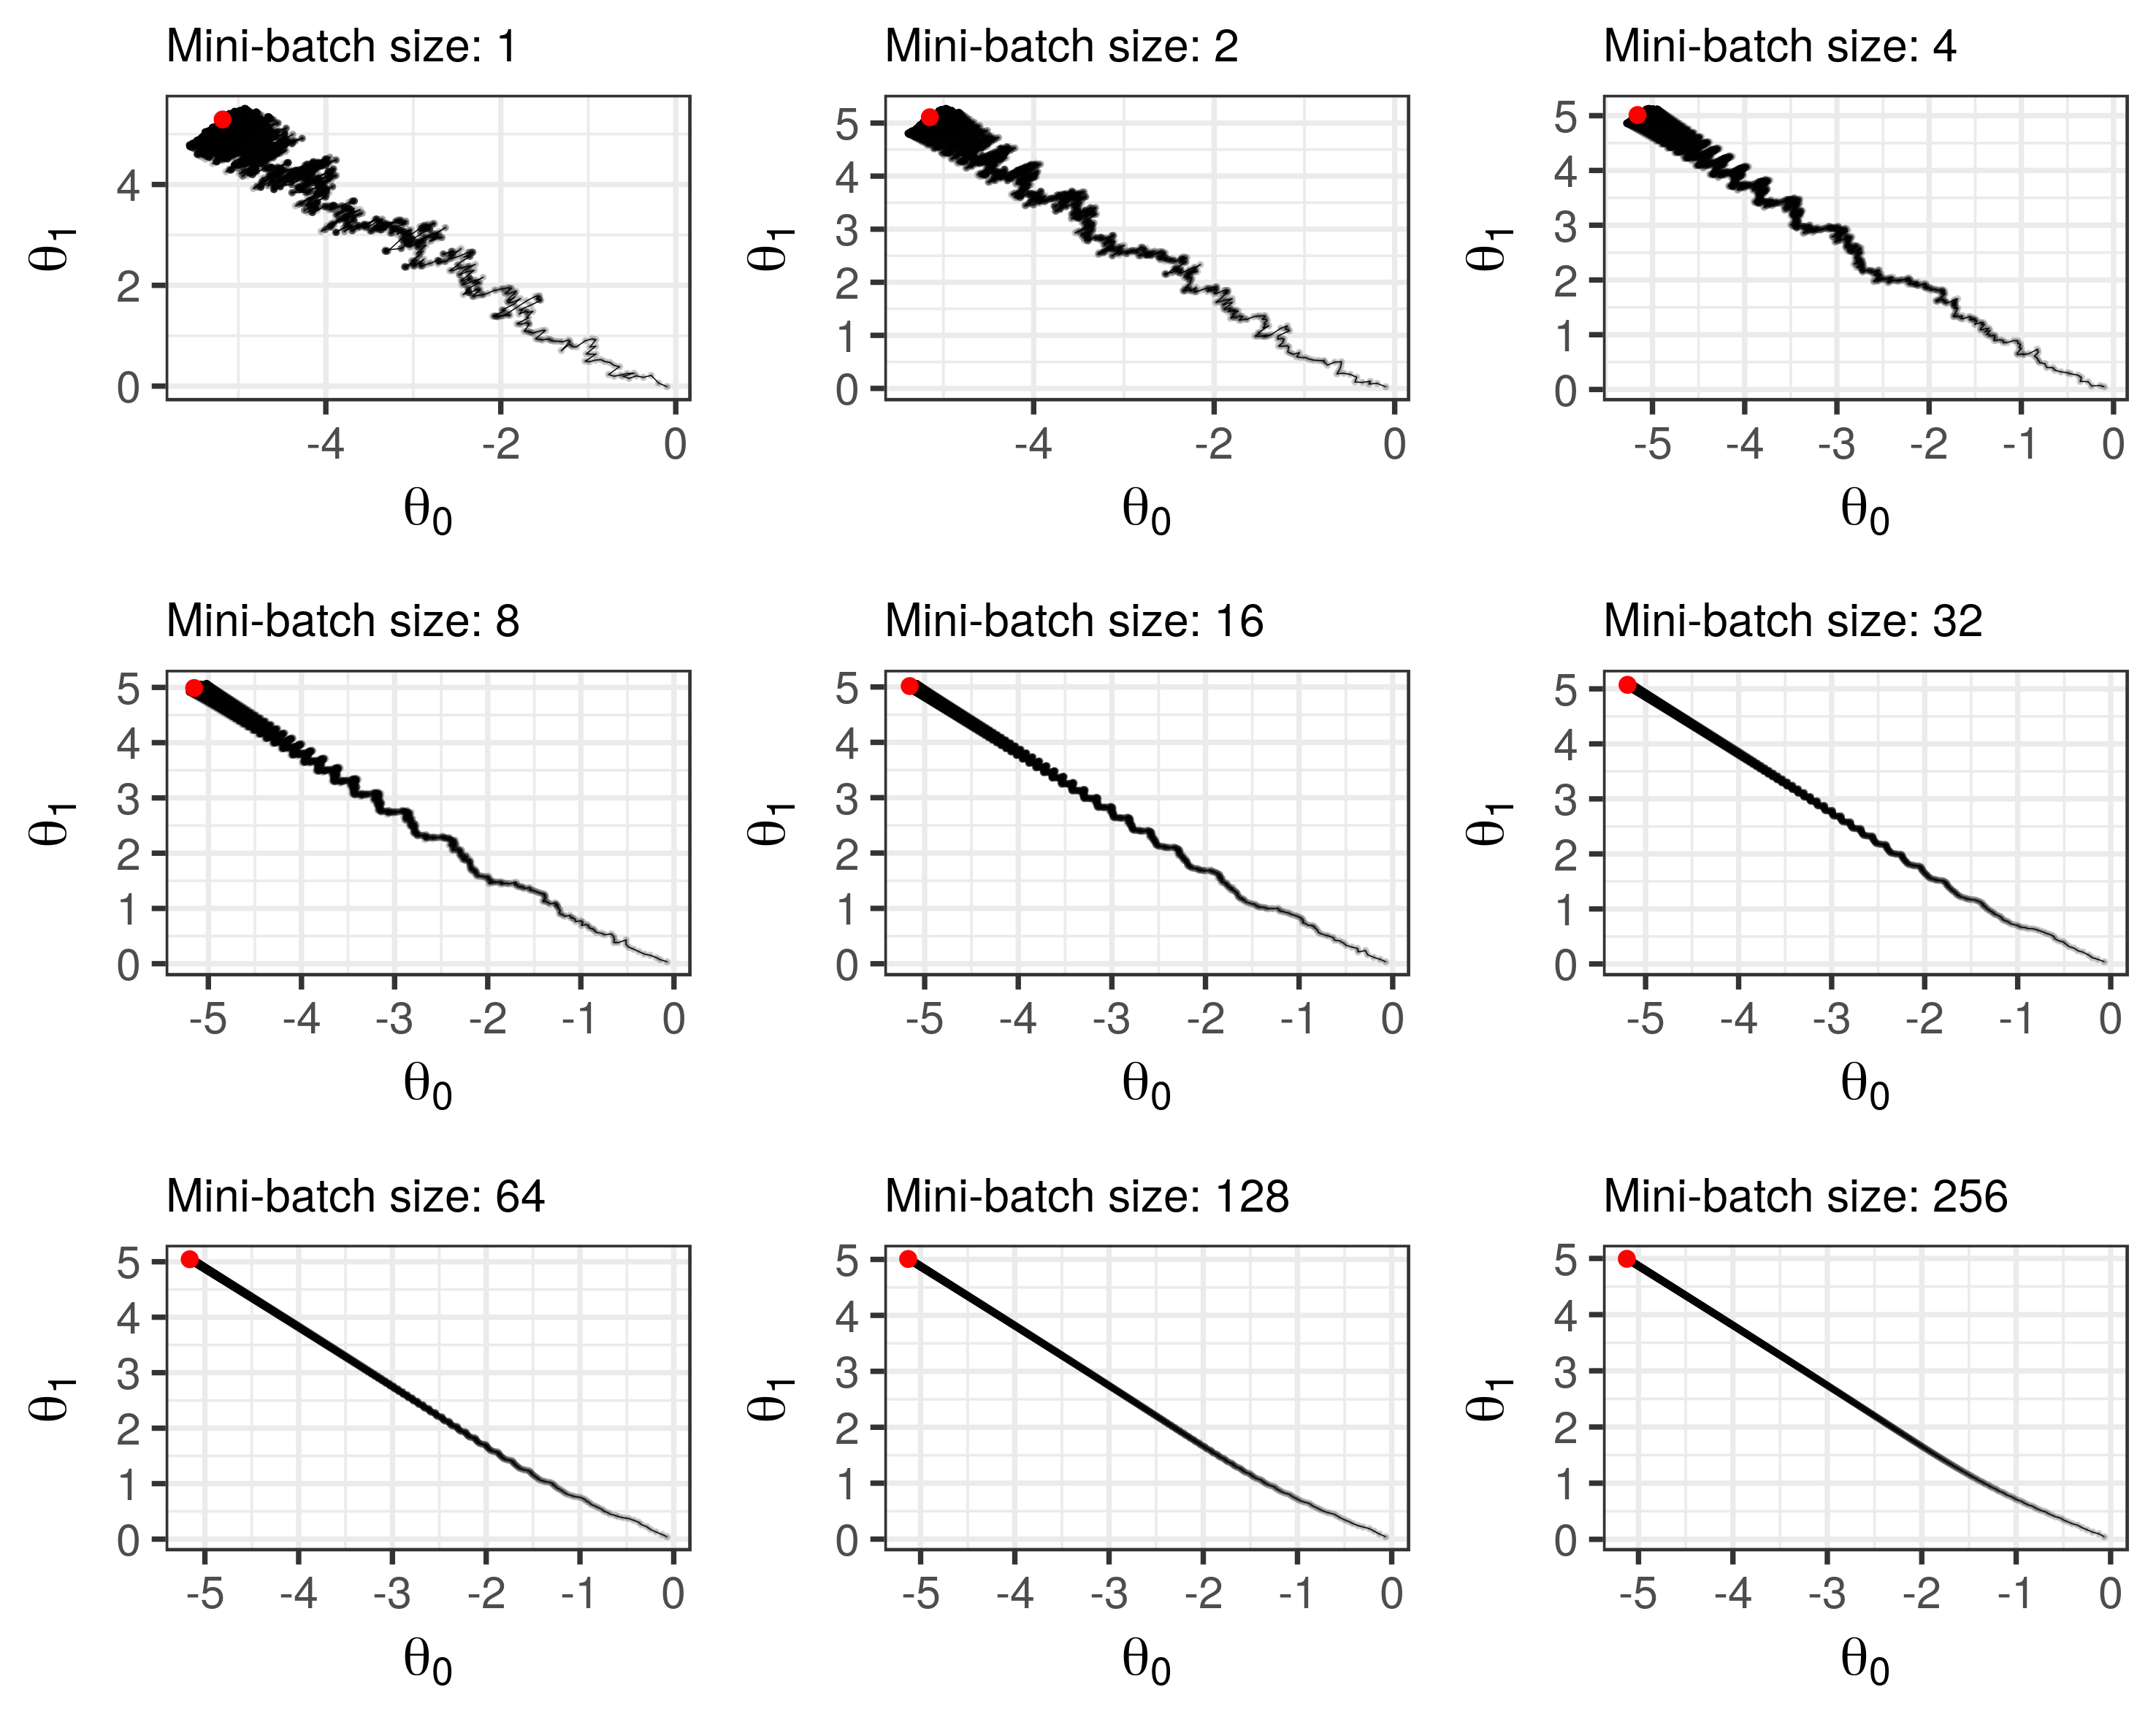
\includegraphics[width=\textwidth]{Mini-batch_GD_plots.png}
    \caption{Example of mini-batch gradient descent for logistic regression comparing mini-batch sizes.}
    \label{fig:Mini-batch_GD_plots}
\end{figure}


\subsection{Overfitting and regularization}

A common problem in machine learning can be \textbf{overfitting}. To explain this, consider the case of modeling a response variable $Y$ with the general model proposed in equation \eqref{eq:general_learning_model}. If $f$ is too flexible, then a larger number of parameters must be estimated, which leads to part of the error being captured by those parameters. This is what is known as overfitting. The problem with an overfit model is that it will give bad predictions with data that has not been previously observed. This is why overfit models have a small training error, but a bigger test error.

One way to control overfitting is with \textbf{regularization}, in which a penalization term is added to the loss function to prevent the parameters from taking values that are too high. A very simple regularizer is the $L_2$ norm regularizer in which the sum of the squared parameters is added to the loss function.

For example, in linear regression, the usual loss function that is sought to be minimized is
\begin{equation}
  \label{eq:lin_reg_loss_funct}
  \sum_{i = 1}^n{ \left( y_i - \sum_{k = 1}^p  \theta_k x_k \right) ^ 2},
\end{equation}
but with the $L_2$ regularizer (also known as ridge regression), equation \eqref{eq:lin_reg_loss_funct} is modified so that the loss function now is
\begin{equation}
  \label{eq:lin_reg_loss_funct_reg}
  \sum_{i = 1}^n{ \left( y_i - \sum_{k = 1}^p \theta_k x_k \right) ^ 2}
  + \lambda \left( \sum_{k = 2}^p \theta_k^2 \right),
\end{equation}
where $\lambda > 0$ is called the regularization parameter, and controls the relative importance between the two main terms of the sum. The value of this parameter can have a big impact in the loss function: if it is too big, then it will penalize too much and most parameters will be near 0, but if it is too small, then there is little regularization effect and it is as if there were no penalization at all. In practice, it is common to choose several concrete values of $\lambda$ (such as 0.001, 0.01 and 0.1) and select the final value using the validation set previously mentioned, so that the final chosen value of $\lambda$ minimizes the validation set error.

Another type of regularization that is widely used in neural network literature nowadays is \textbf{dropout} \cite{srivastava2014dropout}. Dropout consists in randomly dropping out, that is temporarily removing, units of the neural network in each feed-forward mini-batch pass, which results in a thinned network. Each unit is removed, along with all its input and output connections, with a certain probability $p$. The original idea of dropout is that by randomly dropping units, the modeler is essentially training different networks, so the end result is the combination of different architectures, which result in less overfitting. At test time, the prediction is usually just the average of the different thinned networks.

In \citeyear{gal2015dropout1}, \citeauthor{gal2015dropout1} proved that dropout can be seen as a Bayesian approximation to a deep Gaussian process \cite{gal2015dropout}. They show that applying dropout before each weight layer in a neural network with arbitrary depth is mathematically equivalent to a variational approximation that minimized the KL divergence to the posterior distribution to a deep Gaussian process. They later showed that stochastic regularization techniques such as dropout, can be seen as variational approximations to a Bayesian neural network, including convolutional neural networks \cite{gal2015bayesian} \cite{gal2015modern}.
